\subsubsection{Update der Haupt-API}
Bei einem Update der Haupt-API hat die Docker-Compose-Umgebung in jedem Testlauf den Score 35 von 100 erzielt, während die k3s-Umgebung mit dem Score 70 von 100 in jedem Testlauf das Doppelte erreicht hat.
In der Tabelle \ref{tab:chaos_api_update} benötigte die Docker-Compose-Umgebung im Durchschnitt 21,38 Sekunden, um den Service wiederherzustellen, während es bei der k3s-Umgebung zu keinem Ausfall kam.
\begin{table}[htbp]
\centering
\caption{Vergleich der Chaos-Test-Metriken bei Update der Haupt-API}
\label{tab:chaos_api_update}

\begin{tabular}{lrr}
\toprule
\textbf{Metrik} & \textbf{Docker} & \textbf{K3s} \\
\midrule
Error Rate [\%]                    & 7.76 & 3.12 \\
Availability [\%]                & 92.24 & 96.88 \\
Recovery Time [s]       & 21.38 & 0.00 \\
Recovered [Anzahl]  & 3 & 3 \\
\bottomrule
\end{tabular}

\end{table}

\begin{figure}[htbp]
\centering
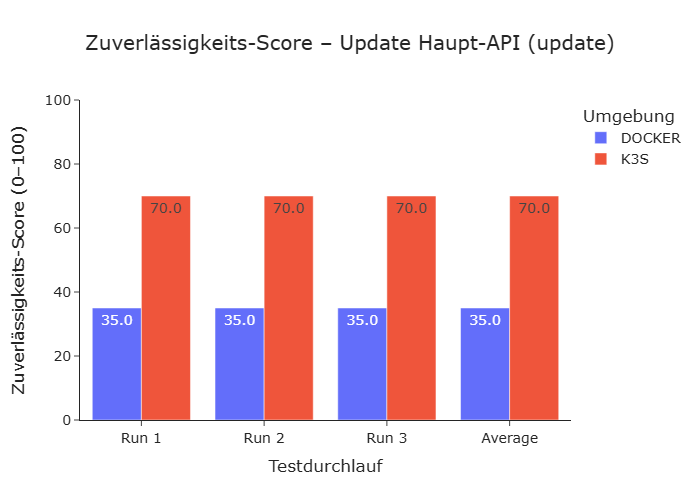
\includegraphics[width=0.8\textwidth]{bilder/tests/reliability_score_api-update_update.png}
\caption{Zuverlässigkeit Score bei Update der Haupt-API}
\label{fig:chaos_api_update}
\end{figure}
\FloatBarrier